\documentclass[10pt,twocolumn,a4paper]{article}
\usepackage[margin=1.6cm,top=1.4cm,bottom=1.6cm]{geometry}
\usepackage{amsmath,amssymb}
\usepackage{graphicx}
\usepackage{booktabs}
\usepackage[hidelinks]{hyperref}
\usepackage{caption}
\usepackage{titlesec}
\usepackage{enumitem}
\captionsetup{font=small,labelfont=bf,skip=3pt}
\titlespacing*{\section}{0pt}{5pt}{2pt}
\titleformat{\section}{\normalsize\bfseries}{\thesection}{0.6em}{}
\setlength{\columnsep}{0.55cm}
\setlength{\textfloatsep}{6pt}
\setlength{\floatsep}{5pt}
\setlength{\dbltextfloatsep}{6pt}
\setlength{\parskip}{1pt}
\setlist{nosep,leftmargin=1.1em}

\title{\vspace{-0.9cm}\textbf{Reducing Bus Bunching on a Loop Route\\with Q-Learning Holding Control}}
\author{Faiz Imdad (B23CM1016)\\
\small GitHub: \url{https://github.com/Faizimdad/bus-bunching-rl}}
\date{\vspace{-0.9cm}}

\begin{document}
\maketitle

\section{Problem}
On frequent bus routes, buses that start evenly spaced drift into \emph{bunches}.
A slightly late bus finds more waiting passengers, dwells longer and falls further
behind, while the bus behind it finds fewer passengers and catches up. Passengers
then wait for a long gap followed by several buses arriving together. Agencies
counter this by \emph{holding} buses at stops, but holding also delays the people
on board. We cast the holding decision as a reinforcement-learning problem: at each
stop, an agent decides whether to hold a bus for 0, 2 or 4 minutes.

\section{Environment}
We built a time-stepped simulator ($\Delta t=0.1$\,min) from scratch. A loop route
has $N{=}12$ stops served by $M{=}4$ buses (capacity 70). Segment run times are
log-normal (mean 2.5\,min, CV 0.25), resampled every departure. Passengers arrive at
each stop as a Poisson process ($\lambda=0.6$\,pax/min); each on-board passenger
alights at a stop with probability 0.15. Dwell time is
$d=0.25+0.08\,n_{\text{board}}+0.04\,n_{\text{alight}}$\,min, and passengers who
arrive while the bus is dwelling or held also board. This dwell feedback alone
reproduces bunching: with no control, 46\% of arrivals at stops follow the previous
bus by less than a quarter of the mean headway (Fig.~\ref{fig:ts}, left). Episodes
last 240\,min; the first 30\,min (warm-up) are excluded from all metrics. Initial
positions are perturbed by up to $\pm15\%$ of the ideal spacing.

\section{RL Formulation}
\textbf{Decision epochs.} A decision is made whenever a bus has finished boarding
and is ready to depart; the interval between decisions is variable, so this is a
semi-Markov decision process. All buses share one policy (parameter sharing),
giving $\approx$\,1{,}100 decisions per episode.

\textbf{State space $S$.} For bus $i$ at a decision we observe
$g_f$, the spatial gap to the bus ahead, and $g_b$, the gap to the bus behind,
both divided by the ideal spacing $N/M$ (so $g=1$ is perfect), plus the load
fraction $\ell=\text{load}/C$. Each gap is discretised into 7 bins with edges
$\{0.3,0.6,0.85,1.15,1.4,1.7\}$ and the load into 3 bins (edges 0.3, 0.6), giving
$|S|=7\times7\times3=147$ discrete states.

\textbf{Action space $A$.} Discrete: hold $h\in\{0,2,4\}$\,min ($|A|=3$).

\textbf{Reward $R$.} The cost of an action is realised when the same bus reaches
its next stop and observes new gaps $g_f',g_b'$:
\begin{equation}
r = -\tfrac{1}{2}\big[(g_f'-1)^2+(g_b'-1)^2\big] \;-\; w_h\,h\,(0.5+\ell),
\end{equation}
with gaps clipped at 2.5 and $w_h=0.05$. The first term rewards even spacing in
both directions; the second penalises holding, more so when many passengers are on
board (the constant 0.5 represents the slower route cycle that holding causes even
for an empty bus).

\textbf{Algorithm.} Tabular Q-learning~\cite{wd,sb},
$Q(s,a)\leftarrow Q(s,a)+\alpha[r+\gamma\max_{a'}Q(s',a')-Q(s,a)]$, where $s'$ is
the state at the same bus's next decision. We use $\alpha=0.1$, $\gamma=0.9$, and
$\varepsilon$-greedy exploration with $\varepsilon$ decaying linearly from 1.0 to
0.05 over the first 70\% of 3{,}000 training episodes (each with a fresh random
seed). The state is small and interpretable, so a table is sufficient and lets us
inspect the policy directly (Fig.~\ref{fig:pol}); a DQN would be the natural next
step for continuous states.

\textbf{Baselines.} All use the same action set. (i) \emph{No holding}.
(ii) \emph{Forward-headway rule}: if $g_f<0.8$, hold for the largest option not
exceeding the time needed to restore $0.8\times$ the ideal gap. (iii) \emph{Two-way
rule}: hold for the largest option not exceeding $\tfrac12(g_b-g_f)$ converted to
minutes, which moves the bus toward the midpoint between its neighbours (a discretised form of headway-based control~\cite{dag}).

\begin{figure*}[t]
\centering
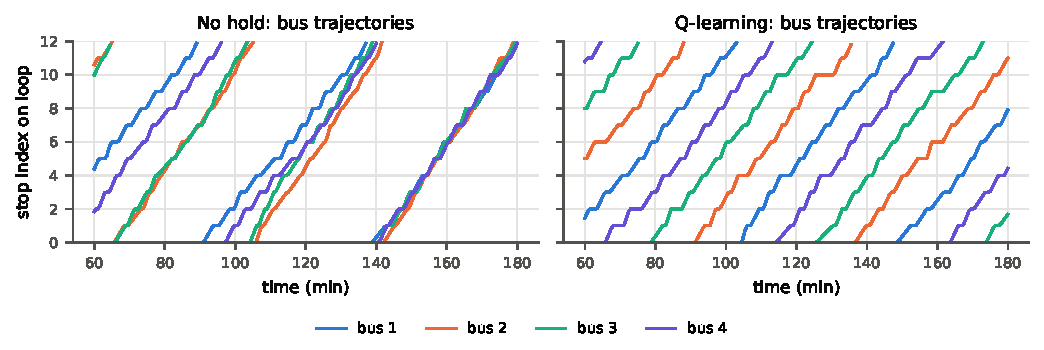
\includegraphics[width=0.92\textwidth]{../results/figures/time_space.pdf}
\caption{Bus trajectories on the same test episode (each line is one bus; flat
steps are dwell/hold). Without control the four buses collapse into one or two
platoons; the learned policy keeps them evenly spaced.}
\label{fig:ts}
\end{figure*}

\begin{figure*}[t]
\centering
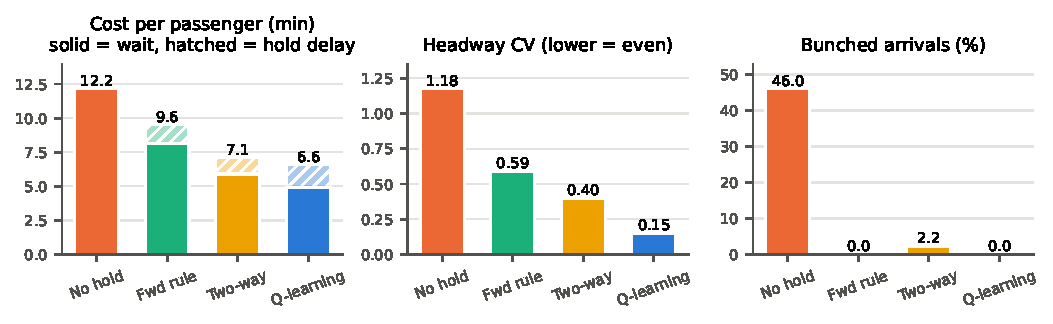
\includegraphics[width=0.92\textwidth]{../results/figures/comparison.pdf}
\caption{Test results averaged over 100 held-out episodes. Left: passenger cost
split into waiting at stops (solid) and delay caused by holding (hatched).}
\label{fig:cmp}
\end{figure*}

\section{Results}
All controllers are evaluated on the same 100 test seeds, disjoint from training
and validation seeds. Table~\ref{tab:res} and Fig.~\ref{fig:cmp} summarise them.
We measure \emph{total cost per passenger} = average wait at stops + held
passenger-minutes per boarding, so a controller cannot look good merely by holding
buses for long periods.

\begin{table}[h]
\centering\small
\setlength{\tabcolsep}{3.2pt}
\begin{tabular}{lccccc}
\toprule
Controller & Wait & Hold & Total & CV & Bunch\% \\
\midrule
No holding      & 12.16 & 0.00 & 12.16 & 1.175 & 46.0 \\
Forward rule    & 8.13  & 1.43 & 9.56  & 0.593 & 0.0 \\
Two-way rule    & 5.90  & 1.23 & 7.14  & 0.401 & 2.2 \\
\textbf{Q-learning} & \textbf{4.91} & 1.68 & \textbf{6.59} & \textbf{0.147} & \textbf{0.0} \\
\bottomrule
\end{tabular}
\caption{Mean over 100 test episodes (minutes per passenger; CV = coefficient of
variation of headways at stops).}
\label{tab:res}
\end{table}

The learned policy cuts total passenger cost by 46\% versus no holding and by 8\%
versus the best rule, and reduces headway CV by $2.7\times$ relative to the two-way
rule. It holds slightly more than the rules (higher hold delay) but buys a much
larger reduction in waiting. Learning is stable: the greedy policy beats the
two-way rule on validation seeds from about episode 1{,}500 onward and the mean
reward plateaus after $\sim$2{,}200 episodes (curves in the repository,
\texttt{results/figures/learning\_curve.png}).

\textbf{What was learned.} Fig.~\ref{fig:pol} shows the greedy action at high
load. The agent holds when the gap ahead is small and the gap behind is large (the
lower-right region), and does not hold when the bus is itself late (large $g_f$,
small $g_b$, upper-left). This mirrors the logic of the two-way rule, but the agent
learns \emph{how much} to hold for each combination from experience rather than
from a fixed formula, and it holds for the full 4\,min more readily when the bus
behind is far away.

\begin{figure}[t]
\centering
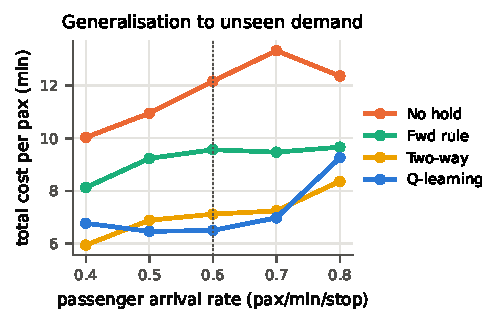
\includegraphics[width=\columnwidth]{../results/figures/sensitivity.pdf}
\caption{Total cost per passenger as demand varies; the agent was trained only at
$\lambda=0.6$ (dotted line). 40 test seeds per point.}
\label{fig:sens}
\end{figure}

\textbf{Generalisation and robustness.} Without retraining, the policy remains the
best controller at $\lambda=0.5$ and 0.7 (Fig.~\ref{fig:sens}). At very light
demand ($\lambda=0.4$) the two-way rule is slightly better, because bunching is
mild and the agent's holds become unnecessary; at heavy demand ($\lambda=0.8$) loads
fall outside the training distribution and the two-way rule again does better.
Training over a range of demand levels would address both cases.
Retraining with four further seeds gives total costs of 6.61--6.77\,min (headway CV
0.147--0.151; 50 test seeds each), all below the two-way rule, so the result is not
a lucky seed. The holding penalty matters: with $w_h=0$ the agent learns to hold
almost always (total cost 26.7\,min). Raising $w_h$ from 0.02 to 0.5 trades
regularity for less holding (CV 0.148$\to$0.292, total cost 6.61$\to$6.43\,min);
operators can set $w_h$ to match how they value on-board delay.

\begin{figure}[t]
\centering
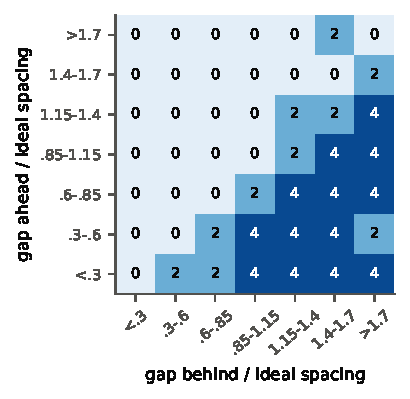
\includegraphics[width=0.82\columnwidth]{../results/figures/policy_high.pdf}
\caption{Learned hold (min) at high load ($\ell>0.6$) as a function of the gap
ahead and the gap behind.}
\label{fig:pol}
\end{figure}

\section{Conclusion and Limitations}
A 147-state Q-learning agent with three actions learns a holding policy that
eliminates bunching and lowers total passenger cost below well-known rule-based
controllers on a stochastic loop route. Limitations: the simulator is synthetic
(not calibrated to a real city), all buses share one policy without
communication, and performance degrades under demand far outside training. Natural
extensions are training across a range of demand levels, a DQN over continuous
gaps, and multi-agent coordination between neighbouring buses.

\begin{thebibliography}{9}\small
\bibitem{sb} R.~S. Sutton and A.~G. Barto, \emph{Reinforcement Learning: An Introduction}, 2nd ed., MIT Press, 2018.
\bibitem{wd} C.~J.~C.~H. Watkins and P.~Dayan, ``Q-learning,'' \emph{Machine Learning}, 8(3--4):279--292, 1992.
\bibitem{dag} C.~F. Daganzo, ``A headway-based approach to eliminate bus bunching,'' \emph{Transportation Research Part B}, 43(10):913--921, 2009.
\end{thebibliography}

\end{document}
